
\chapter{Teilautomatisierte Generierung von Page Objects}
\label{sec:teilautomatisierte_generierung_von_pageObjects}

Ein großer Teil des in Kapitel \ref{sec:probleme_des_page_object_pattern} angesprochenen initialen Mehraufwands, bei der Verwendung des Page Object Pattern beläuft sich auf die Erstellung der Page Object Klassen.
Wie in Listing \ref{lst:poCreatePage} und \ref{lst:poShowPage} zu sehen ist, sind Page Objects nicht sehr komplex. In der Praxis zeigt sich, dass ein Großteil der Arbeit darin besteht, die verschiedenen Lokatoren der Elemente aus dem Quelltext der Seite zu extrahieren und in die generische Form eines Page Objects zu überführen.
Diese Aufgabe kostet zwar viel Zeit, ist allerdings nicht sehr anspruchsvoll.
Möchte man den initialen Mehraufwand bei der Verwendung des Page Object Pattern entgegenwirken, liefern die Page Objects somit einen guten Ansatzpunkt.
Aufgrund ihrer generischen Natur bieten sie gute Voraussetzungen, um automatisch generiert zu werden.
\section{Übersicht über die Idee}
\label{sec:uebersicht_ueber_idee}


Selenium, in Verbindung mit dem Page Object Pattern, ist auch ein Teil des Technologiestacks des IT-Dienstleisters der Landeshauptstadt München (it@M) und wird dort zum Testen komplexer Webanwendungen verwendet. Auch it@M hat in Bezug auf die Erstellung von Page Objects die Erfahrung gemacht, dass es sich um eine generische und zeitaufwendige Arbeit handelt.
In Zusammenarbeit wurde daher die Idee entwickelt, das Erstellen von Page Objects mit Hilfe einer Softwarelösung zu unterstützen.
Anhand des Seitenquelltextes der zu testenden Webanwendung sollen die verschiedenen Elemente des Page Objects identifiziert und zur Generierung der Klassen verwendet werden.
Zwei Ansätze wurden dabei diskutiert. Eine vollautomatisierte und eine teilautomatisierte Generierung von Page Objects.\\
Ein vollautomatischer Ansatz würde beinhalten, dass ohne weiteres Zutun aus dem Seitenquelltext ein vollständiges Page Object generiert wird. Dieser Ansatz hat jedoch mit zahlreichen Problemen zu kämpfen. Oft wird nur ein Bruchteil der Elemente einer Webseite für die Testfälle benötigt. Selenium kann aber prinzipiell jedes Element, dass im Seitenquelltext bereitgestellt wird, ansprechen. Bei einer vollautomatischen Generierung müssten daher entweder alle Elemente einer Seite übernommen, oder eine definierte Auswahl getroffen werden.
Wird eine Auswahl getroffen, besteht das Risiko, dass Elemente ausgelassen werden, die vom Tester möglicherweise benötigt werden. Werden alle Elemente übernommen, werden die Page Objects schnell überfüllt und unübersichtlich. Das Überfüllen der Page Objects geschieht dann auf Kosten ihrer Robustheit. Strukturelle Änderungen in der Website wirken sich auch auf die Lokatoren der Elemente aus. Um die Page Objects stabil zu halten, müssen diese bei Änderungen in der Seitenstruktur berichtigt werden.
Es ist daher nicht sinnvoll, Elemente in den Page Objects zu pflegen, die nicht verwendet werden. Unbenutzte Elemente bedeuten entweder zusätzlichen Wartungsaufwand oder veralten unbemerkt.\\
Ein weiteres Problem des vollautomatischen Ansatzes stellen die Übergänge zwischen den Seiten einer Webanwendung dar. Interaktionen, wie beispielsweise das Betätigen eines Links oder Button, führen oft zum Aufrufen einer neuen Seite der zu testenden Webanwendung. Im weiteren werden diese Übergänge als Transitionen bezeichnet. Diese Transitionen werden auch in den Page Objects abgebildet. Das Page Object gibt dazu das entsprechende Page Object der Zielseite als Rückgabe eines Methodenaufrufs der Ausgangsseite zurück. In der Methode \grq CreatePage.createEntry()\grq\ im Listing \ref{lst:poCreatePage} ist diese Vorgehen dargestellt. Allein aus dem Seitenquelltext zu ermitteln, welche Seite das Ziel einer Transition ist, erweist sich oft als sehr schwierig bis unmöglich.\\
Um die Komplexität des Projektes aufgrund der genannten Probleme nicht zu groß werden zu lassen, entschied man sich für eine teilautomatisierte Lösung.
Ziel ist es also nicht, ein vollständiges Page Object vollautomatisiert zu generieren, sondern den Entwickler bei der Generierung der Page Objects zu unterstützen. Anhand des Quelltextes sollen dem Entwickler die möglichen Elemente der Seite in einer Vorauswahl bereitgestellt werden. Aus diesen Elementen können dann diejenigen ausgewählt werden, die im späteren Page Object benötigt werden. Auf diese Weise wird ein Überladen verhindert und gleichzeitig sichergestellt, dass die Elemente, die benötigt werden, vorhanden sind.
Ob es sich bei einem Element um eine Transition handelt, also ein Element, welches auf eine neue Seite führt, muss nicht mehr automatisch anhand des Quelltextes ermittelt werden, sondern wird vom Entwickler direkt bei der Auswahl der benötigten Elemente mit angegeben.
Die so vom Entwickler ausgewählten Informationen können später verwendet werden, um daraus das fertige Page Object zu generieren.
Im Rahmen des Projektes \grq SeleniPo\grq\ soll dieser Ansatz in Zusammenarbeit mit it@M in Form einer Desktopanwendung umgesetzt werden. 

\section{Abgrenzung zu bestehenden Ansätzen}
\label{sec:abgrenzung_zu_bestehenden_ansaetzen}
Sowohl für die vollautomatische Generierung von Page Objects, als auch für eine teilautomatisierte Generierung, gibt es bereits mögliche Lösungsansätze. 
Stocco et al. \cite{stocco_why_2015} beschreiben in einem Paper das von ihnen entwickelte Framework APOGEN, mit deren Hilfe Page Objects vollautomatisch generiert werden können. Die Generierung geht dabei weit über das Anlegen von Elementen hinaus und schließt auch die Funktionalitäten der einzelnen Webseiten in Form von Methoden mit ein.
Das Framework analysiert dazu die Struktur der Webanwendung mittels eines Crawlers. Die Informationen, die über den Crawler zusammengetragen wurden, wie beispielsweise das DOM der einzelnen Webseiten, werden anschließend über eine statische Analyse aufbereitet und für die Generierung der Page Objects verwendet.
Nach Angaben der Forschungsgruppe sollen ca. 75\% des von APOGEN generierten Codes ohne Anpassungen verwendet werden können. Die restlichen 25\% benötigen nur kleine Änderungen.\\
Bei APOGEN handelt es sich jedoch um ein noch sehr junges Projekt. Das entsprechende Paper wurde im Mai 2015 veröffentlicht. APOGEN ist daher eher ein Prototyp, der zwar die Möglichkeiten aufzeigt, die in diesem Bereich gegeben sind, jedoch noch nicht für den produktiven Einsatz in einem großen Unternehmen geeignet ist.
Nach eigenen Angaben leidet das Projekt noch unter einigen Einschränkungen. Eine der genannten Einschränkungen ist die Limitierung durch den Crawler.
APOGEN kann nur Webseiten in Page Objects umwandeln, die auch durch den Crawler erreicht werden.
Für einfache Webanwendungen stellt das kein großes Problem dar, für sehr komplexe Anwendungen mit einer ausgeprägten logischen Validierung allerdings schon.
Viele Seiten, die hinter logisch validierten Eingaben liegen, können vom Crawler nicht erreicht werden und stehen somit für die Generierung nicht zur Verfügung.\\
Neben der vollautomatischen Generierung existieren noch eine Reihe von Open-Source-Framworks,
die einen teilautomatisierten Ansatz verfolgen, ähnlich wie es das Projekt SeleniPo erreichen will.
Stocco et al. \cite{stocco_why_2015} nennen in ihrem Paper die drei derzeit wichtigsten Vertreter:

\begin{itemize}
\item \textit{OHMAP} \cite{virtuetech_gmbh_ohmap_2015}: Bei OHMAP handelt es sich um eine Webseite, die es dem Benutzer erlaubt, HTML-Code in eine Textarea zu kopieren. Aus dem übergebenen HTML-Code generiert das Tool eine einfache Java-Klasse, die für jedes gefundene Input-Feld ein WebElement enthält. Die Variablennamen werden dabei aus den HTML-Attributen gebildet. Als Lokator wird ein einfacher XPath-Ausdruck verwendet.
	
\item \textit{SWD Page Recorder} \cite{dmytro_zharii_dzharii/swd-recorder_2015}: Der SWD Page Recorder ermöglicht es dem Benutzer eine beliebige Webanwendung zu starten und das GUI der Anwendung mit einem \grq click\&record\grq-Mechanismus zu inspizieren.
Nach jedem Klick auf das Interface der Anwendung wird ein Dropdown-Menü angezeigt, in welches manuell ein Name für das ausgewählte Element eingetragen werden kann. Als Lokator wird ein einfacher XPath-Ausdruck generiert.
Das so erstellte Modell der Anwendung kann in verschiedene Sprachen exportiert werden, wie beispielsweise Java, C\#, Python, Ruby oder Perl. Beim SWD Page Recorder handelt es sich um eine .NET Anwendung.

\item\textit{ WTF PageObject Utility Chrome Extension} \cite{daniel_wiredrive/wtframework_2015}: WTF unterstützt den Entwickler beim Erstellen von Page Objects, indem Lokatoren der Form id, name, CSS oder XPath erstellt werden. Der Code wird in Python generiert.
	
\end{itemize}

Der Technologiestack von it@M sieht eine Entwicklung der Selenium-Testfälle in Java vor. Als Betriebssystem kommt darüber hinaus Linux zum Einsatz.
Zwei der genannten Lösungsansätze scheiden mit dieser Einschränkung für den produktiven Einsatz beim IT-Dienstleister der Landeshauptstadt München aus. Beim SWD Page Recorder handelt es sich um eine .NET Anwendung, die nur schwer unter Linux betrieben werden kann. Die WTF PageObject Utility Chrome Extension kann nur im Python-Umfeld betrieben werden. OHMAP wäre aus technischer Sicht eine mögliche Lösungsalternative. Allerdings sind Komfort und Umfang der Anwendung aus Sicht von it@M nicht ausreichend. Ohne eigene Konfiguration ist es mit OHMAP nur möglich, input-Felder zu erkennen.
Darüber hinaus muss der HTML-Quelltext händisch aus der zu testenden Anwendung extrahiert werden. \\
Sowohl OHMAP, als auch der SWD Page Recorder haben zusätzlich das Problem, dass die erzeugten XPath Ausdrücke oft sehr einfach gewählt werden und damit sehr stark von der Position der Elemente innerhalb der Seite abhängig sind. Die eigentlichen Charakteristika der Elemente werden oft nicht beachtet. Listing \ref{lst:badXPath}
zeigt einen solche von OHMAP generierten XPath.

\begin{lstlisting}[caption={Einfacher XPath-Lokator des Projektes OHMAP},label={lst:badXPath}]
	public class YourPageObjectName {
		//...		
 		@FindBy(xpath = "/html/body/div/div[1]/div[1]/h1/a[2]")
		public WebElement followVirtuetechGmbH;	
		//...
	}
\end{lstlisting}

Der zu adressierende Link in Listing \ref{lst:badXPath} wird alleine über seine Position innerhalb des DOM der Seite bestimmt.
Um den Lokator zu zerstören würde es genügen, ein weiteres div-Tag vor dem Link einzufügen. Bezieht man den XPath auf die eigentlichen Charakteristika, wie beispielsweise ein id-Attribut, können sehr viel stabilere Ausdrücke erzeugt werden.
\\
Negativ ist an allen gezeigten Lösungen, dass sie immer nur ein Page Object auf einmal betrachten. Transitionen, also Übergänge zwischen den einzelnen Webseiten der zu testenden Anwendung, werden nicht beachtet. Die dynamische Komponente der Anwendung wird beim Generieren der Page Objects außer Acht gelassen und muss nachträglich händisch hinzugefügt werden.

Mit SeleniPo soll der Versuch unternommen werden, die Schwachstellen der bereits existierenden Lösungsansätzen zu verbessern und eine plattformunabhängige Lösung zu schaffen, die in der IT-Infrastruktur von it@M ausgeführt werden kann.

\newpage
\section{SeleniPo - Page Object Generator}
\label{sec:selenipo_pogenerator}

Abbildung \ref{fig:poGenerator} zeigt die Denktopanwendung (Page Object Generator), die im Rahmen des Projektes SeleniPo entwickelt wurde. Mit Hilfe dieser Anwendung können Page Objects teilautomatisiert generiert werden. Es wird dazu die Möglichkeit geboten, einen Browser zu starten und über vorgefertigte Selektoren die Webanwendung nach benötigten Elementen bzw. Transitionen zu durchsuchen. Auf diese Weise kann ein Modell der Anwendung erstellt werden, dass zur Generierung der Page Objects verwendet wird.

\begin{figure}[htb]
  \centering  
  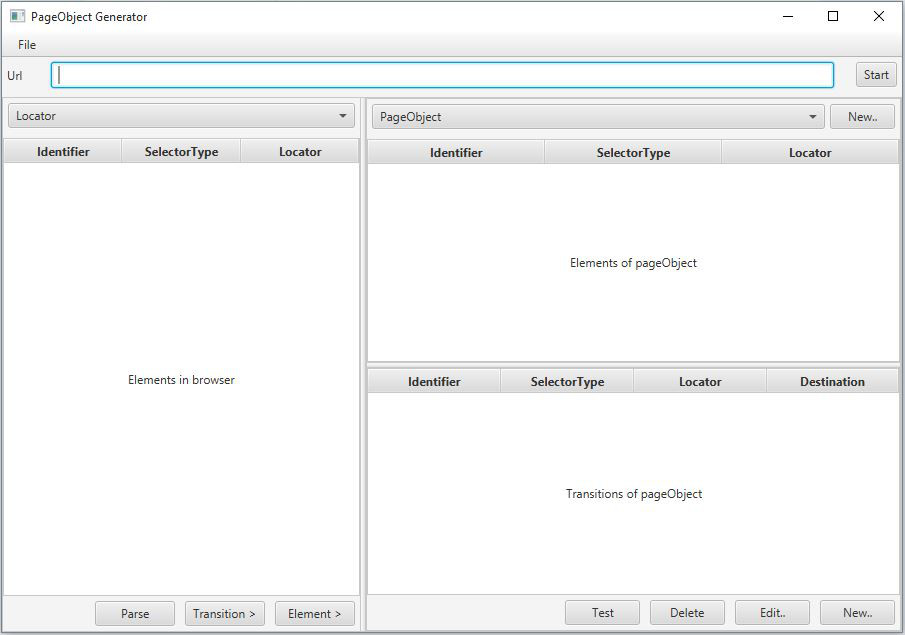
\includegraphics[scale=0.5]{img/poGenerator.JPG}\\
  \caption{SeleniPo - Page Object Generator}
  \label{fig:poGenerator}
\end{figure}



Die Benutzeroberfläche des Page Object Generators teilt sich in drei Bereiche:

\begin{itemize}
	\item Das aktuelle Page Object Modell (Abbildung \ref{fig:poGeneratorPo})
	\item Den HTML-Parser (Abbildung \ref{fig:poGeneratorHtml})
	\item Das Menü (Abbildung \ref{fig:poGeneratorMenu})
\end{itemize}


Abbildung \ref{fig:poGeneratorPo} zeigt den Bereich des Generators, mit dem das aktuelle Page Object Modell der zu testenden Anwendung verwaltet werden kann. Mit diesem Teil der Anwendung können neue Page Objects angelegt und bearbeitet werden. Elemente und Transitionen können manuell hinzugefügt, editiert oder gelöscht werden. Darüber hinaus besteht die die Möglichkeit, existierende Elemente und Transitionen auf ihre Richtigkeit zu testen.

\begin{figure}[htb]
  \centering  
  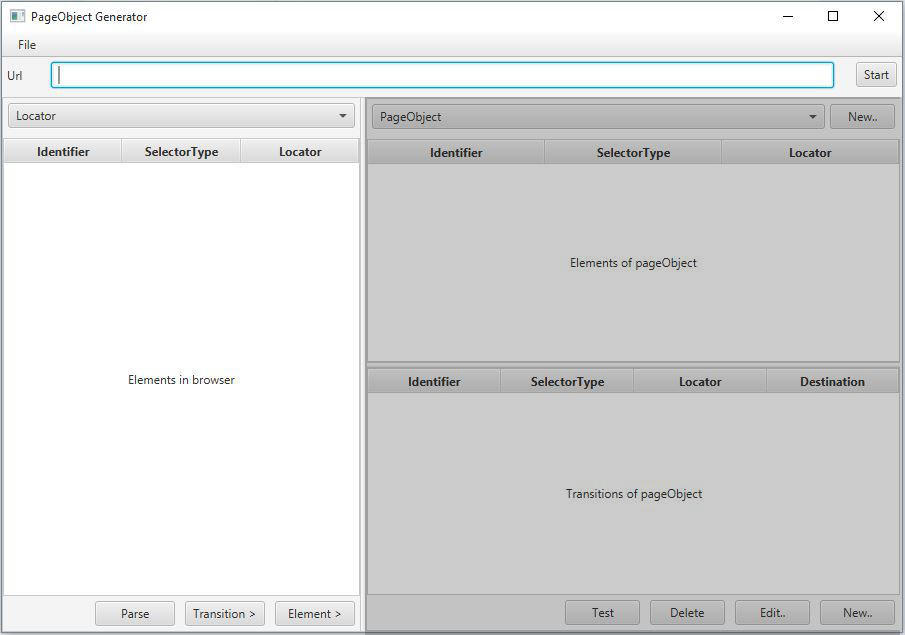
\includegraphics[scale=0.5]{img/poGeneratorPo.JPG}\\
  \caption{SeleniPo - Page Object Generator - Page Object Model}
  \label{fig:poGeneratorPo}
\end{figure}

\newpage

Abbildung \ref{fig:poGeneratorHtml} zeigt den Bereich des Generators, mit dem der Entwickler bei der Erstellung von Elementen und Transitionen im Page Object unterstützt werden kann.
Über den Start-Button kann ein Browser gestartet werden. Über das Lokator-Dropdown kann mittels vorgefertigten Selektoren die aktuell im Browser dargestellte Webseite nach Elementen bzw. Transitionen durchsucht werden. Im Page Object benötigte Elemente und Transitionen können dann in das ausgewählte Page Object übernommen werden, um so ein Page Object Modell der zu testenden Webanwendung zu erstellen.

\begin{figure}[htb]
  \centering  
  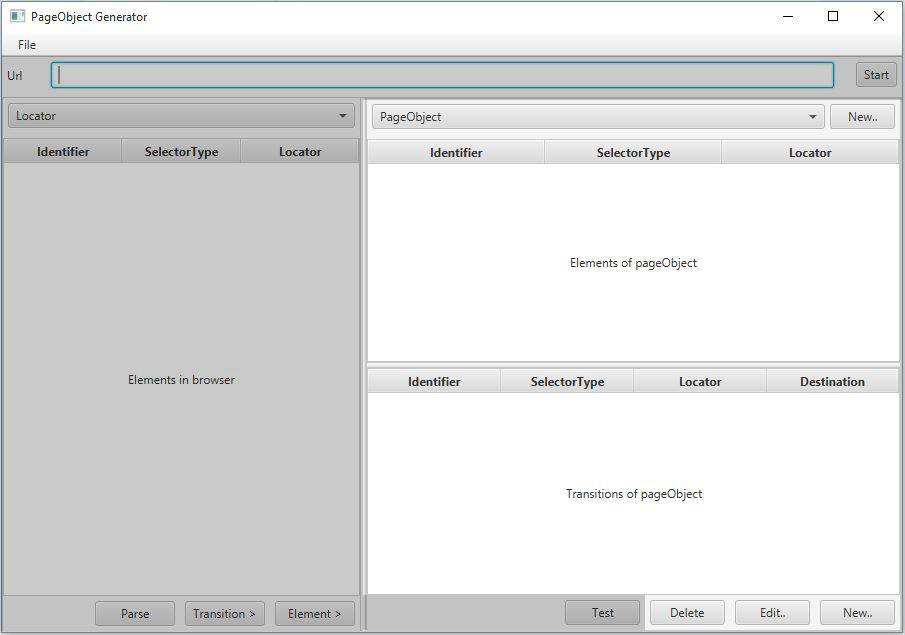
\includegraphics[scale=0.5]{img/poGeneratorHtml.JPG}\\
  \caption{SeleniPo - Page Object Generator - HTML Parser}
  \label{fig:poGeneratorHtml}
\end{figure}

\newpage

Abbildung \ref{fig:poGeneratorMenu} markiert das Menü des Page Object Generators. Mit Hilfe des Menüs können Zwischenstände des Page Object Modells gespeichert und geladen werden.
Über das Menü wird auch die Generierung der Page Objects aus dem aktuell geladenen Modell ausgelöst.

\begin{figure}[htb]
  \centering  
  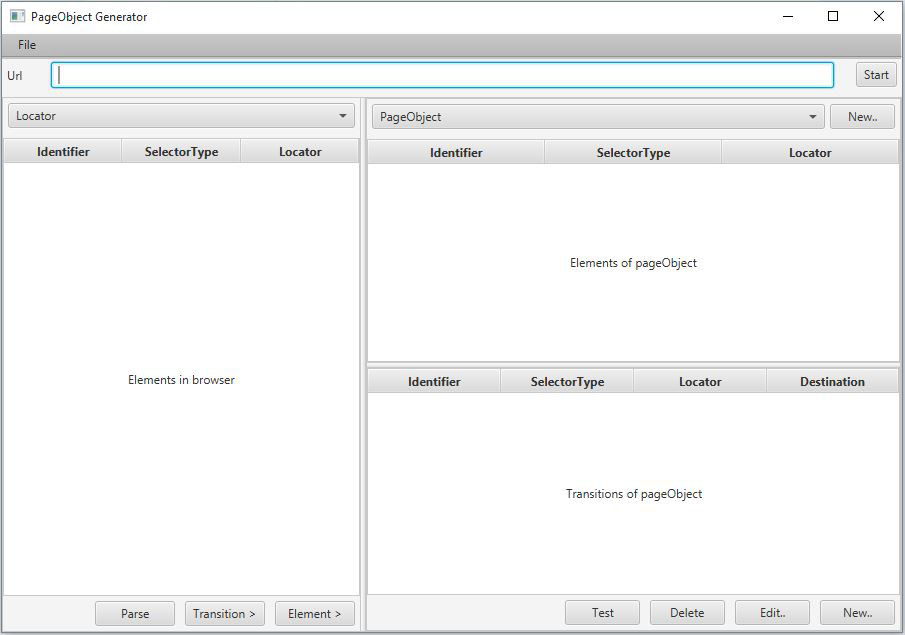
\includegraphics[scale=0.5]{img/poGeneratorMenu.JPG}\\
  \caption{SeleniPo - Page Object Generator - Menü}
  \label{fig:poGeneratorMenu}
\end{figure}

\subsection{Einordnung des Page Object Generator in den Gesamtkontext}
\label{sec:deploymentsicht}


Abbildung \ref{fig:deployment} zeigt die Einordnung des Page Object Generator in die Infrastruktur von it@M. Anhand dieser Abbildung soll gezeigt werden, in welchem Bezug sich der Generator zu einer zu testenden Webanwendung und dem späteren Testprojekt befindet.

\begin{figure}[htb]
  \centering  
  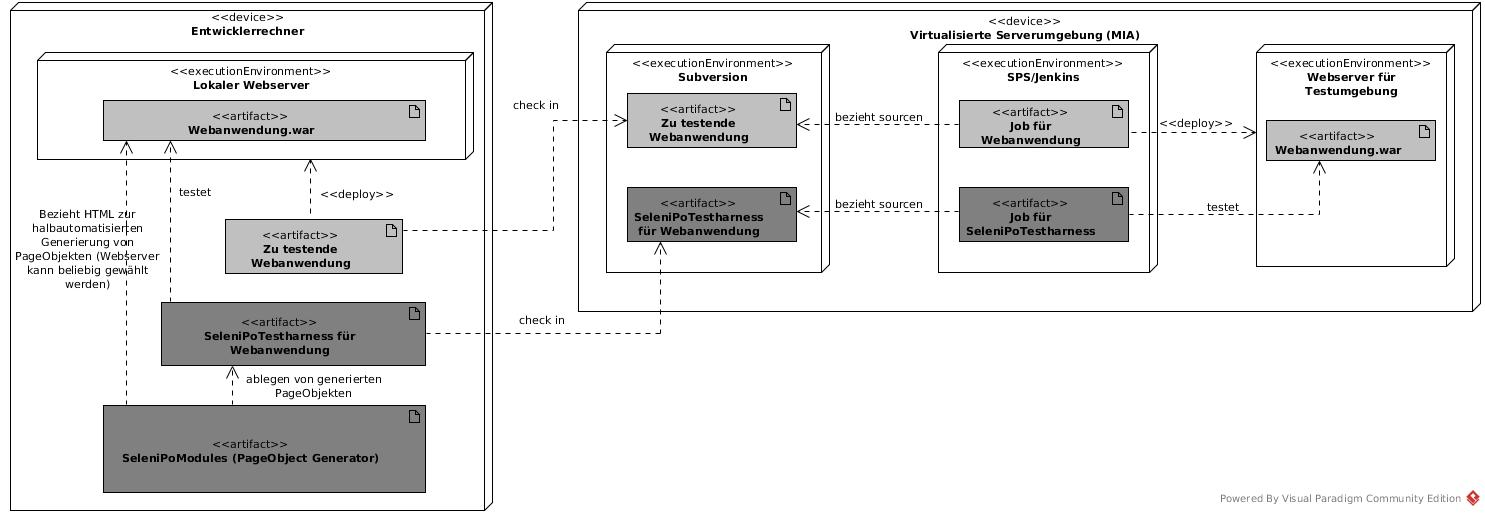
\includegraphics[scale=0.45]{img/Deployment.jpg}\\
  \caption{Einordnung des Page Object Generator in die Deploymentsicht}
  \label{fig:deployment}
\end{figure}

Zwei übergeordnete Teilbereiche werden unterschieden. Die virtualisierte Serverumgebung (MIA) und der lokale Rechner eines Entwicklers.\\
Auf der virtualisierten Serverumgebung werden die entwicklerübergreifenden Infrastrukturkomponenten, wie beispielsweise eine Versionsverwaltung, bereitgestellt. Unter dem Entwicklungsrechner ist der Arbeitsplatz eines einzelnen Projektteilnehmers zu verstehen.\\
Auf dem Entwicklungsrechner wird die zu testende Webanwendung entwickelt. Zu Testzwecken kann diese Anwendung, in ihrem aktuellen Entwicklungsstand, auf einem lokalen Webserver bereitgestellt werden.
Der lokale Rechner des Entwicklers ist darüber hinaus auch der Ort, an dem der Page Object Generator eingesetzt wird. Die vom Entwickler lokal bereitgestellte Webanwendung kann verwendet werden, um für die verschiedenen Seiten der zu testenden Anwendung Page Objects mit Hilfe des Generators zu erzeugen. Diese Page Objects werden in ein Test-Projekt abgelegt, in welchem später auch die Selenium-Testfälle entwickelt werden. In Abbildung \ref{fig:deployment} wird dieses Projekt als SeleniPoTestharness bezeichnet und kann vom Entwicklerteam entweder selbst erstellt oder als leeres Quickstart-Projekt vorgefertigt bezogen werden.\\ 
Mit Hilfe der Page Objects im Testharness können Testfälle entwickelt werden, die während der Erstellung auf dem lokalen Entwicklungsrechner, gegen die lokal bereitgestellte Webanwendung ausgeführt werden.\\
Über die virtualisierte Serverumgebung werden die lokal erstellten Ergebnisse zusammengeführt. 
Der Sourcecode der zu testende Webanwendung, sowie des SeleniPoTestharness, wird in einer Versionsverwaltung in der MIA abgelegt. Bei it@M kommt zu diesem Zweck \grq Subversion\grq\ zum Einsatz.\\
Über die Versionsverwaltung kann dann ein Integration Server bedient werden, der das Bauen, Bereitstellen und Testen der Webanwendung automatisiert. It@M verwendet hierfür den Continuous Integration Server \grq Jenkins\grq\ in Verbindung mit Maven und einem Artifactory.\\
Jenkins bezieht die jeweils aktuellen Sourcen für das Testprojekt und die Webanwendung aus der Versionsverwaltung. So kann regelmäßig eine aktuelle Version der Webanwendung gebaut und auf einem Testsystem in der virtuellen Serverumgebung bereitgestellt werden. Gegen dieses Testsystem können dann mit Hilfe des Jenkins-Servers die im Testharness entwickelten Selenium Testfälle zur Ausführung gebracht werden.



\subsection{Beispielhafter Ablauf bei der Benutzung des Page Object Generators}
\label{sec:moeglicher_ablauf_eines_standartanwendungsfall}

Abbildung \ref{fig:sequenz} zeigt auf hoher Abstraktionsebene einen Standardablauf bei der Benutzung des Page Object Generators.



\begin{figure}[htb]
  \centering  
  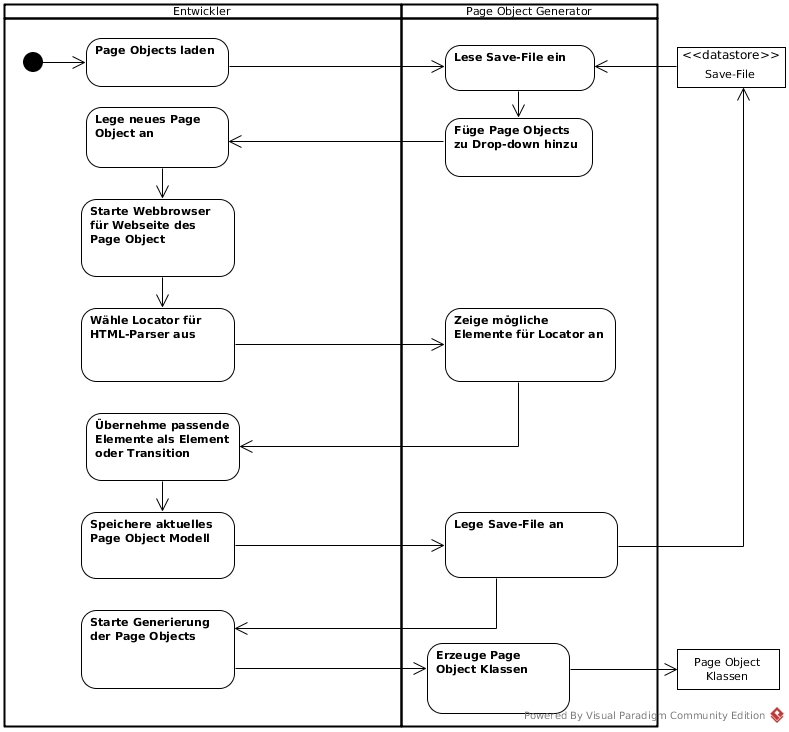
\includegraphics[scale=0.45]{img/Activitydiagram.jpg}\\
  \caption{Beispielhafter Ablauf bei der Benutzung des Page Object Generator}
  \label{fig:sequenz}
\end{figure}

Über das Menü (siehe Abbildung \ref{fig:poGeneratorMenu}) hat der Benutzer des Page Object Generators die Möglichkeit, einen bereits zuvor angelegten Zwischenstand des Page Object Modells aus einem Save-File zu laden. Die bereits angelegten Page Objects werden nach dem Laden im Dropdown-Menü im Bereich des Page Object Modells (siehe Abbildung \ref{fig:poGeneratorPo}) angezeigt. Der Benutzer hat nun die Möglichkeit, mit den bereits vorhandenen Page Objects weiterzuarbeiten oder ein neues Page Object anzulegen. Entscheidet er sich ein neues Page Object anzulegen, wird dies im Dropdown-Menü vorausgewählt angezeigt. Das Page Object kann nun manuell mit Elemente bzw. Transitionen befüllt werden.\\ Um das Page Object jedoch teilautomatisiert zu befüllen wird ein Webbrowser gestartet. Im Browser muss die Seite der Webanwendung aufgerufen werden, die dem aktuell ausgewählten Page Object entspricht. Mit dem Dropdown des HTML-Parser (siehe Abbildung \ref{fig:poGeneratorHtml}) wird die ausgewählte Webseite nach Elementen bzw. Transitionen durchsucht.
Passende Ergebnisse können dann in das ausgewählte Page Object übernommen und dort bei Bedarf noch einmal überarbeitet werden.
Der neu generierte Zwischenstand wird wiederum über das Menü gespeichert.\\
Um die Page Objects letztendlich als Code aus dem Modell zu erzeugen, kann über das Menü die Generierung gestartet werden. Bei richtiger Konfiguration des Page Object Generators muss dazu lediglich das Rootverzeichnis des entsprechenden Testprojektes als Zielort der Generierung gewählt werden.


\subsection{Anwendungsfälle des Page Object Generator}
\label{sec:page_object_generator_usecases}

Die konkreten Anwendungsfälle des Page Object Generators sind in Abbildung \ref{fig:use_case} dargestellt.

\begin{figure}[htb]
  \centering  
  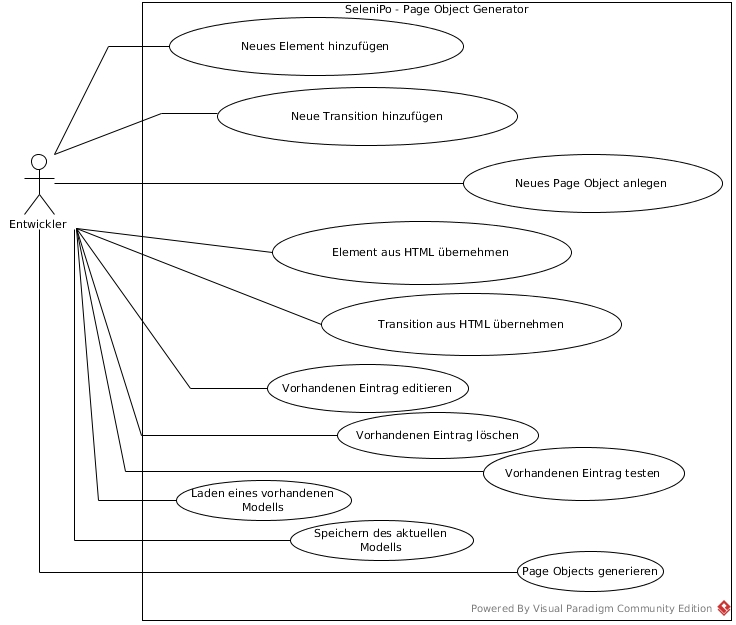
\includegraphics[scale=0.45]{img/Use-Cases.jpg}\\
  \caption{Anwendungsfälle des Page Object Generators}
  \label{fig:use_case}
\end{figure}

Eine detailierte Ausformulierung der Anwendungsfälle befindet sich im Anhang \ref{anhang:anwendungsfallbeschreibung}

\newpage

\subsection{Aufbau und technische Aspekte der Anwendung}
\label{sec:aufbau_des_systems}
In seiner internen Struktur ist der Page Object Generator in vier Module aufgeteilt, die unterschiedliche Aufgaben übernehmen. Diese Module sind auf Projektebene in einem übergeordneten Modul mit dem Namen \grq SeleniPoModules\grq\ zusammengefasst. Abbildung \ref{fig:component_diagramm} zeigt die verschiedenen Module und deren Abhängigkeiten zueinander.
Neben den Modulen des Page Object Generators zeigt Abbildung \ref{fig:component_diagramm} zusätzlich den SeleniPoTestharness, der dazu verwendet werden kann, die vom Page Object Generator erzeugten Klassen in einen ausführbaren Kontext zu stellen.\\
Im Folgenden wird auf die Aufgaben der einzelnen Module kurz näher eingegangen.

\begin{figure}[htb]
  \centering  
  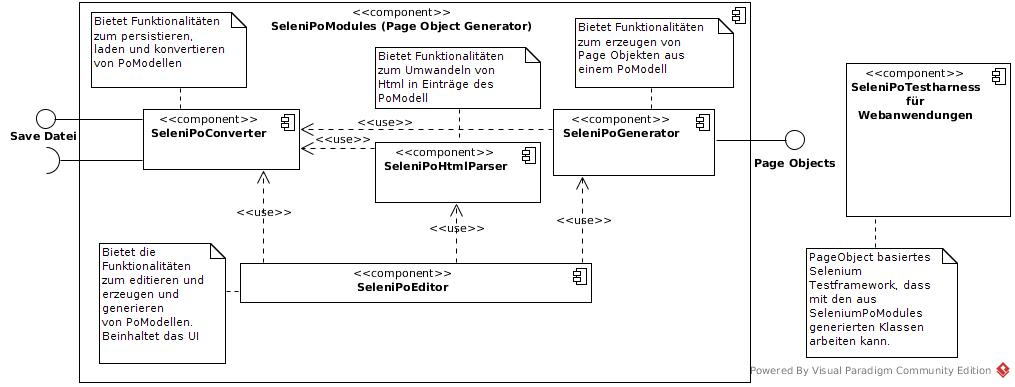
\includegraphics[scale=0.46]{img/ComponentDiagram.jpg}\\
  \caption{Module des Page Object Generators}
  \label{fig:component_diagramm}
\end{figure}

\subsubsection{SeleniPoEditor}
\label{sec:selenipoeditor}

Das zentrale Modul des Page Object Generators ist der SeleniPoEditor.
Ausgehend von diesem Modul werden die übrigen Module verwendet, um die in Kapitel \ref{sec:page_object_generator_usecases} vorgestellten Anwendungsfälle zu verwirklichen.
Das Modul SeleniPoEditor stellt dazu die grafische Benutzeroberfläche (GUI) der Anwendung bereit.
Als Technologie wird hierbei JavaFX \cite{oracle_client_2015} verwendet, das mit der Java Version 8 Einzug in den Oracle JDK gefunden hat. \\
Um eine hohe Wartbarkeit dieser Komponente zu gewährleisten, wurde die GUI nach dem Model-View-Controller Prinzip verwirklicht.
Das Modell besteht aus einem anwendungsspezifischem Java Objekt, welches eine Liste von Page Objekten mit deren zugehörigen Attributen darstellt.
Für die View wird die XML-basierte Sprache FXML verwendet, um losgelöst von der Applikationslogik die Struktur der Benutzeroberfläche zu beschreiben.
Der Controller besteht aus Java Klassen, mit deren Hilfe das Verhalten der GUI bei Benutzerinteraktion beschrieben wird.
Komplexere Logik, wie beispielsweise das Generieren der fertigen Page Object Klassen wird mittels Services durch die übrigen Modulen bereitgestellt.\\
Das Verhalten der GUI wird über einen Zustandsautomaten gesteuert.
Interaktionen mit der Oberfläche beeinflussen den Zustand, in dem sich die Anwendung befindet. Je nach Zustand variieren die Aktionen, die von den verschiedenen Buttons der Anwendung ausgelöst werden.
Mit Hilfe dieses Vorgehens kann beispielsweise beim Editieren nach der Auswahl eines Elements, ein anderer Dialog angezeigt werden, als nach der Auswahl einer Transition.
Die verschiedenen Zustände der GUI, sowie die Events, die in diesen Zuständen verarbeitet werden, sind im Anhang \ref{sec:zustände_des_page_object_generator} über einen erweiterten endlichen Automaten dargestellt.

\subsubsection{SeleniPoConverter}
\label{sec:selenipoconverter}
Das Modul SeleniPoConverter dient der Verwaltung des internen Modells des Page Object Generators. In dieser Komponente wird einerseits das Modell der Anwendung definiert, andererseits werden Services für andere Module bereitgestellt, um mit diesem Modell zu arbeiten.
Abbildung \ref{fig:simple_model} zeigt die Interface-Stuktur, welche das Modell abbildet.

\begin{figure}[htb]
  \centering  
  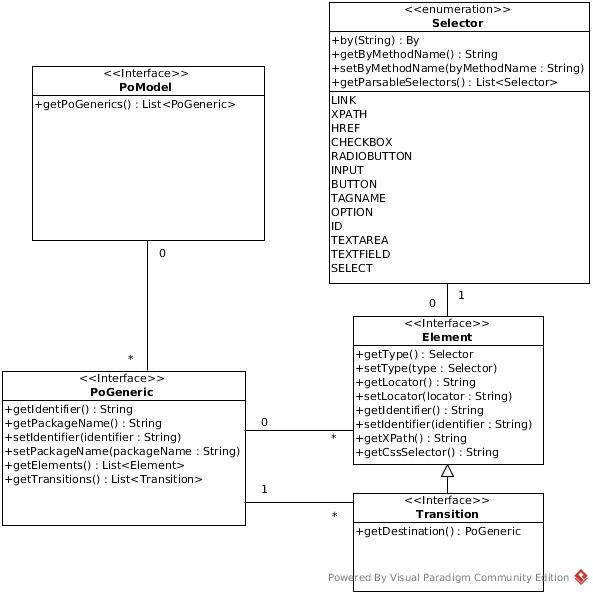
\includegraphics[scale=0.46]{img/SimpleModel.jpg}\\
  \caption{Vereinfachte Struktur des internen Modells des Page Object Generators}
  \label{fig:simple_model}
\end{figure}

Kern des Modells ist das Interface PoModel, welches eine Liste von PoGenerics beinhaltet. Ein PoGeneric repräsentiert die Informationen, die benötigt werden, um eine einzelne Page Object Klasse zu erzeugen. Dementsprechend vereint dieses Interface eine Menge an Elementen und Transitionen.
Ein Element steht dabei für eine beliebige Komponente einer Webseite, wie beispielsweise ein Eingabefeld.
Transitionen sind von Elementen abgeleitet. Es handelt sich also um eine speziellere Form von Elementen. Mit Hilfe von Transitionen ist es möglich, auch die dynamische Komponente einer Webseite in Form von Seitenübergängen abzubilden. Als Transition werden all die Komponenten einer Webseite bezeichnet, die einen Übergang auf ein neues Page Object auslösen. Im Gegensatz zu Elementen bieten Transitionen daher noch ein Page Object Ziel mit an. Über die Methode \grq getDestination()\grq\ kann dieses Page Object Ziel erfragt werden\\
Sowohl Elemente als auch Transitionen werden über eine Selektor-Enumeration genauer definiert.
Der Selektor gibt für ein Element im Modell an, welche Suchstrategie beim Auflösen des Lokators gegen die Webseite verwendet werden soll.
Die verfügbaren Strategien werden durch die verschiedenen Aufzählungstypen der Enumeration festgelegt.\\
Die Kerninformation zum Adressieren eines Elements auf der Webseite bildet der Lokator. Vom Generator wird diese Variable mit einem Wert befüllt, der charakteristisch für das zu adressierende Element ist. Je nach Element handelt es sich hierbei oft um ein HTML-Attribut, wie beispielsweise id- oder value-Attribute des entsprechenden HTML-Tags.\\
In Verbindung mit dem ausgewählten Selektor kann über eine selbst erstellte Klasse \grq ByFactory\grq\ aus dem Lokator ein repräsentativer XPath-Ausdruck bzw. CSS-Selektor für das Element erzeugt werden. Im Kapitel \ref{sec:selenipotestharness} wird darauf näher eingegangen.\\
Abbildung \ref{fig:simple_model} zeigt lediglich die Interface-Struktur des zugrunde liegenden Modells. Der Page Object Generator kennt zwei konkrete Implementierungen. Das vollständige Modell ist in Anhang \ref{anhang:vollständiges_technisches_modell} abgebildet.\\
Zwei verschiedene Implementierungen sind notwendig, da JavaFX und XStream \cite{joe_walnes_xstream_2015}, welches für die Persistierung in XML verwendet wird, unterschiedliche Anforderungen an das Modell stellen. JavaFX benötigt spezielle Datentypen. Anstelle einer gewöhnlichen List wird beispielsweise eine ObservableList verwendet, um die View der GUI automatisch mit dem Modell synchron zu halten. Diese Datentypen können von XStream aufgrund eines fehlenden argumentlosen Konstruktors jedoch nicht mehr deserialisiert werden.
Dementsprechend werden vom Converter eine Reihe von Services bereitgestellt, die das Wandeln des Modells in zwei Implementierungen ermöglicht. Eine Implementierung kann verwendet werden, um das Modell zu persistieren und wieder zu deserialisieren. Die Zweite Implementierung wird verwendet um im Umfeld von JavaFX zu arbeiten.\\
Abbildung \ref{fig:converter_service} zeigt alle vom Converter bereitgestellten Services. 

\begin{figure}[htb]
  \centering  
  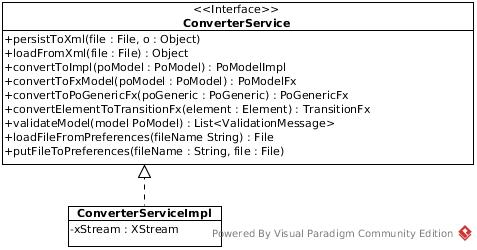
\includegraphics[scale=0.5]{img/ConverterService.jpg}\\
  \caption{Services, die von SeleniPoConverter bereitgestellt werden}
  \label{fig:converter_service}
\end{figure}

Neben den Services zum Wandeln des Modells wird in diesem Modul auch die Funktionalität zum Speichern und Laden, sowie zur fachlichen Validierung bereitgestellt.
Zusätzlich wird die Möglichkeit geboten, benutzerspezifische Informationen, wie beispielsweise den Pfad zum zuletzt verwendeten Save-File, in den Properties des Anwenders abzulegen.


\subsubsection{SeleniPoHtmlParser}
\label{sec:selenipohtmlparser}

Das SeleniPoHtmlParser Modul beinhaltet die Funktionalität zum teilautomatisierten befüllen des Page Object Modells mit Elementen bzw. Transitionen.
Das Modul stellt dazu eine Methode bereit, die es ermöglicht HTML-Quelltext anhand von einem übergebenen Selektor auszuwerten.
Abbildung \ref{fig:html_service} zeigt das Klassendiagramm für diesen Service.

\begin{figure}[htb]
  \centering  
  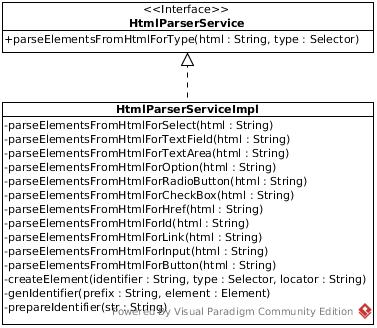
\includegraphics[scale=0.5]{img/HtmlParserService.jpg}\\
  \caption{Services, die von SeleniPoHtmlParser bereitgestellt werden}
  \label{fig:html_service}
\end{figure}

Der benötigte HTML-Quelltext wird direkt aus einem Webbrowser bezogen, der über die Benutzeroberfläche der Anwendung gestartet werden kann.
Das Parsing des Quelltextes übernimmt die freie Bibliothek jsoup \cite{hedley_jsoup_2015}.
Für jeden in der Selektor-Enumeration (siehe Kapitel \ref{sec:selenipoconverter}) definierten Aufzählungstypen wurde dazu eine eigene Strategie implementiert. 
Die für die jeweiligen Selektoren implementierte Filterstrategie orientiert sich an der Strategie, die später in den Testfällen verwendet wird, um die Elemente auf der Webseite zu adressieren.\\
Listing \ref{lst:parserLINK} zeigt beispielhaft die Implementierung für den Aufzählungstypen LINK, der Links auswählt, welche eines der HTML-Attribute id, text oder title besitzen:
\begin{lstlisting}[caption={Parser für den Aufzählungstypen LINK},label={lst:parserLINK}]
 	/**
	 * Sucht nach Links fuer die vorhanden ist: id or text or title
	 *
	 * @param html Quelltext der zu untersuchenden Seite
	 * @return PoGeneric - neues Page Object mit den gefundenen Elementen
	 */
	private PoGeneric parseElementsFromHtmlForLink(String html) {
		final String PREFIX = "a";
		PoGeneric poGeneric = new PoGenericImpl();
		Document doc = Jsoup.parse(html);
		Elements elements = doc.select("a");
		for (Element element : elements) {
			if (element.hasAttr("id")) {
				de.muenchen.selenipo.Element createdElement = createElement(
						genIdentefier(PREFIX, element), Selector.LINK,
						element.attr("id"));
				poGeneric.getElements().add(createdElement);
			}
			else if (element.hasText()) {
				de.muenchen.selenipo.Element createdElement = createElement(
						genIdentefier(PREFIX, element), Selector.LINK,
						element.text());
				poGeneric.getElements().add(createdElement);
			}
			else if (element.hasAttr("title")) {
				de.muenchen.selenipo.Element createdElement = createElement(
						genIdentefier(PREFIX, element), Selector.LINK,
						element.attr("title"));
				poGeneric.getElements().add(createdElement);
			}
		}
		return poGeneric;
	}
  }
  
\end{lstlisting} 

Dieses Vorgehen hat den Nachteil, dass die Möglichkeit besteht, Elemente zu verwerfen, die vom Benutzer für den ausgewählten Filter zwar erwartet werden, den implementierten Filterkriterien jedoch nicht entsprechen.
Im Beispiel aus Listing \ref{lst:parserLINK} wären das alle Links, für die weder das Attribut id, text oder title gesetzt ist.\\
Durch dieses Vorgehen ist allerdings sichergestellt, dass für einen untersuchten Selektor nur Elemente zur Auswahl gestellt werden, die in den späteren Testfällen auch aufgelöst werden können. So wird verhindert, dass über die Page Objects Elemente bereitgestellt werden, die später in den Testfällen zu Fehlern führen.\\
Die Palette der vorgefertigten Filter deckt einen großen Teil der in HTML vorhandenen Elemente bereits ab. Sollte es dennoch vorkommen, dass Elemente über die existierenden Selektoren nicht erreicht werden, besteht die Möglichkeit mit Hilfe des Selektors XPATH, Elemente über einen eigenen XPath-Ausdruck anzusprechen.



\subsubsection{SeleniPoGenerator}
\label{sec:selenipogenerator}
Das Modul SeleniPoGenerator ermöglicht es, aus einem Modell des SeleniPoConverters, Page Object Klassen zu generieren.
Abbildung \ref{fig:generator_service} zeigt die Services, die von diesem Modul angeboten werden.

\begin{figure}[htb]
  \centering  
  \includegraphics[scale=0.5]{img/SelenipoGenerator.jpg}\\
  \caption{Services die von SeleniPoHtmlParser bereitgestellt werden}
  \label{fig:generator_service}
\end{figure}

Für die Generierung des Codes aus dem Modell der Anwendung wird die Template-Engine Velocity \cite{apache_software_foundation_apache_2015} verwendet.
Mit Hilfe von Velocity kann ein beliebiges Modell der Anwendung über vordefinierte Templates in die gewünschten Page Object Klassen gewandelt werden.
Diese Templates können vom Benutzer des Page Object Generators beliebig editiert werden. So ist es möglich, die im Modell der Anwendung hinterlegten Informationen in jede, vom Anwender gewünschte Form aufzubereiten. Anhang \ref{anhang:beispiel_velocity_template} zeigt als Beispiel den Templatevorschlag, der im Rahmen dieser Arbeit im Page Object Generator verwendet wird.\\
Für jedes Page Object im Modell werden jeweils zwei Klassen erzeugt. Eine Klasse, welche die gesamte generierte Logik enthält, sowie eine weitere Klasse, welche abgesehen von einem Konstruktor leer ist und von dieser Klasse ableitet. 
Die komplexe Klasse wird im folgenden als \grq PageObject\_Generated\grq\ bezeichnet. Das zugehörige Template befindet sich in Listing \ref{lst:template_pogenerated}. Die
bis auf den Konstruktor leere Klasse wird im folgenden als \grq PageObject\_Dynamisch\grq\ bezeichnet und ist im Template, in Listing \ref{lst:template_poeditable} dargestellt.\\
Abbildung \ref{fig:postruktur} zeigt die Abhängigkeit zwischen den beiden zu generierenden Klassen.

\begin{figure}[htb]
  \centering  
  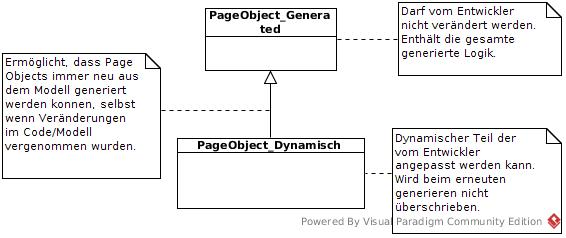
\includegraphics[scale=0.6]{img/postruktur.jpg}\\
  \caption{Abhängigkeit zwischen dem generierten und dem dynamischen Teil eines Page Objects}
  \label{fig:postruktur}
\end{figure}
 
Mit Hilfe der Aufteilung eines Page Objects in zwei Klassen soll verhindert werden, dass bei mehrmaligem Generieren des gleichen Page Objects Änderungen, die vom Testentwickler im Code vorgenommen wurden, überschrieben werden. Als Konvention gilt daher, dass Änderungen durch den Entwickler nur im PageObject\_Dynamisch vorgenommen werden dürfen. Der generierte Teil des Page Objects darf vom Entwickler nicht verändert werden.
Bei einem erneuten generieren der Page Objects werden lediglich die PageObject\_Generated überschrieben, der dynamische Teil bleibt unangetastet.
Dadurch ist sichergestellt, dass Änderungen, die im dynamischen Teil geschehen nicht überschrieben werden, jedoch Anpassungen die über den Page Object Generator vorgenommen wurden, Einzug in den generierten Teil finden können.
Page Objects können so über die gesamte Projektlaufzeit iterativ im Page Object Generator aufgebaut werden und müssen nicht bereits zu Beginn im finalen Zustand modelliert werden.\\
Der Ort an dem die fertigen Page Objects abgelegt werden, ist über eine Konfigurationsdatei und eine Variable in den Page Objects einstellbar. 
Abbildung \ref{fig:packagepath} stellt grafisch dar, wie die endgültige Paket-Struktur eines Page Objects gebildet wird.
\begin{figure}[htb]
  \centering  
  \includegraphics[scale=0.8]{img/packagePath.png}\\
  \caption{Erzeugen der Paket-Struktur eines Page Object}
  \label{fig:packagepath}
\end{figure}
In der Grundkonfiguration wird der generierte Teil eines Page Objects unterhalb des Ordners \grq src.main.generated\grq\ abgelegt. Der dynamische Teil befindet sich unterhalb von \grq src.main.java\grq.
Diese Strukturierung bildet die getroffene Konvention ab, dass bei Verwendung der Page Objects der dynamische teil als Instanz in den Testfällen verwendet wird und der generierte Teil nicht editiert werden darf.
Ausgehend von diesen Verzeichnissen ist es über die Konfiguration möglich, den Pfad weiter zu verfeinern. So kann konfiguriert werden, dass der generierte Teil eines Page Objects immer im Paket \grq de.muenchen.selenipo.po\grq\ abgelegt wird, der dynamische im Paket \grq de.muenchen.selenipo.po\grq.\\
Während der Erstellung im Page Object Generator kann auf Ebene der Page Objects eine weitere Verfeinerung der Struktur vorgenommen werden. Ausgehend von den global konfigurierten Ziel-Paketen ist es so möglich, jedes Page Object in ein beliebiges Paket abzulegen.
Bei richtiger Konfiguration kann dann für die Generierung der Klassen, einfach das Rootverzeichnis des Testprojektes ausgewählt werden.

\subsubsection{SeleniPoTestharness}
\label{sec:selenipotestharness}

Im Rahmen dieser Arbeit wurde auch ein Testprojekt entwickelt, welches mit den Page Objects, die über den Page Object Generator erzeugt wurden, arbeiten kann.
Das Testprojekt wird im folgenden als Testharness bezeichnet.\\
Damit Testharness und Page Object Generator zusammenarbeiten können, muss die Struktur der Templates des Generators mit der Struktur des Testharness zusammenpassen.
Die Struktur der Templates kann vom Benutzer des Page Object Generators jederzeit angepasst werden. Prinzipiell kann dadurch jede Struktur eines Testharness unterstützt werden.\\
Um mit den Templates, die im Rahmen dieser Arbeit entwickelt wurden, zusammenzuarbeiten, muss der Testharness allerdings einige Anforderungen erfüllen.
Abbildung \ref{fig:strukturTestharness} zeigt die Page Object Struktur, die sowohl in den Templates als auch im Testharness verwendet wird.\\
\begin{figure}[htb]
  \centering  
  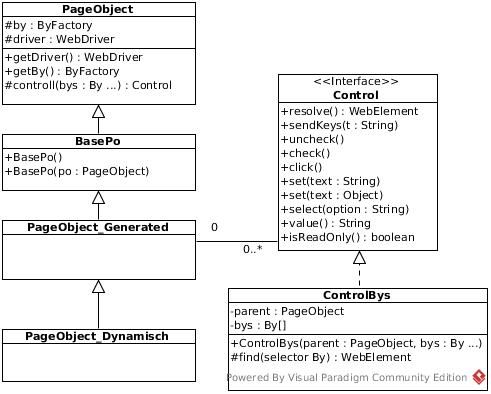
\includegraphics[scale=0.49]{img/strukturTestharness.jpg}\\
  \caption{Page Object Struktur des Testharness}
  \label{fig:strukturTestharness}
\end{figure}

Die Wurzel der Vererbungshierarchie eines Page Objects im Testharness bildet die Klasse PageObject. Die Klasse PageObject beinhaltet den Selenium WebDriver. Neben dem WebDriver enthält die Klasse PageObject noch eine zusätzliche Kernkomponente, die Klasse ByFactory. Diese Klasse zählt nicht zum Standard bei der Verwendung des Page Object Pattern sondern ist spezifisch für die in dieser Arbeit verwirklichte Implementierung eines Testharness.
Die Helferklasse ByFactory ermöglicht es in einfacher Art, komplexe \grq org.openqa.selenium.By\grq -Ausdrücke zu erzeugen. Die erzeugten Ausdrücke werden verwendet, um über den WebDriver Elemente auf der Webseite zu lokalisieren. Als Übergabe erhält die Factory dazu einen einfachen Lokator-String, der beispielsweise dem value- oder id-Attribut des gesuchten HTML-Tags entspricht. Die Klasse ByFactory ist mit dem Page Object Generator abgestimmt. Für jeden Selektor des Generators gibt es eine entsprechende Factory-Methode. Die vom Generator erzeugten Lokatoren sind so gewählt, dass sie von der ByFactory interpretiert werden können. Damit ist sichergestellt, dass ein vom Generator erzeugter Lokator von der entsprechenden Factory-Methode aufgelöst werden kann.\\
Die Verwendung der Factory-Klasse bringt den Vorteil, dass komplexe XPath Ausdrücke einfach erzeugt sowie gekapselt und lesbar in den Page Objects abgelegt werden können. 
Das Modell des Generators bietet auch die Möglichkeit die bereits aufgelösten Ausdrücke, ohne die zusätzliche Verwendung der ByFactory, zu erhalten.
Mit den Methoden  \grq Element.getXPath()\grq\ bzw.  \grq Element.getCssSelector()\grq\ können je nach verwendetem Selektor, der XPath bzw. der CssSelector als String erfragt werden. \\
Die Klasse BasePo ist das nächste Kind in der Vererbungshierarchie. Als einzige Klasse bietet BasePo einen parameterlosen Konstruktor und bildet somit, bei der Verwendung der Page Objekts, den Einstiegspunkt in einen Testfall. Bei der konstruktorlosen Initialisierung des BasePo wird ein neuer WebDriver erzeugt, der auf einer über die Konfiguration hinterlegbaren Adresse startet.
Alle weiteren Page Objects erhalten bei der Instanziierung als Übergabe ein bereits vorhandenes Page Object, aus dem der WebDriver übernommen werden kann.
Damit kann der Zustand des WebDrivers innerhalb eines Testfalls von Page Object zu Page Object übergeben werden.\\
Ausgehend von der Klasse BasePo erben die vom Page Object Generator erzeugten Klassen, PageObject\_Generated und PageObject\_Dynamisch (siehe Kapitel \ref{sec:selenipogenerator}).
Die verschiedenen Elemente der Webseite werden im Page Object als Implementierung des Interfaces Control angeboten.
Die Klasse ControlBys implementiert dieses Interface und kapselt ein Selenium WebElement. Als Referenz gegen die Webseite wird bei der Instanziierung ein By-Ausdruck übergeben, der mittels ByFactory erzeugt werden kann.
Für die Interaktion mit dem referenzierten Element bietet die Klasse eine Vielzahl von Methoden an. Eine davon ist die Methode \grq Control.resolve()\grq, welche das gekapselte WebElement zurückliefert.\\
Die Kapselung eines WebElements in die Klasse ControlBys hat den Vorteil, dass WebElemente in einem Page Object als globale Variablen geführt werden können.
Die Klasse ControlBys verhindert, dass ein WebElement sofort bei der Instanziierung eines Page Object gegen die geladene Webseite im Webdriver aufgelöst wird. Erst beim Aufruf einer Methode wird der übergebene By-Ausdruck verwendet, um das eigentliche WebElement über die WebDriver-Methode \grq findElement()\grq\ zu erhalten.
So wird verhindert, dass ein Page Object bereits bei der Instanziierung versucht, Elemente auf der Webseite abzufragen, die möglicherweise noch gar nicht geladen sind oder erst durch vorangegangene Interaktion erreichbar gemacht werden müssen.\\ Zum einfachen Erzeugen von Controls bietet die Klasse PageObject die statische Methode \grq control(bys : By ...)\grq\ an, die auch in den Templates verwendet wird.


\section{Praxistest}
Um im Praxisbetrieb erste Erfahrungen mit dem Page Object Generator zu sammeln, wurde eine frühe Version des Generators dazu verwendet, Page Objects für ein bereits etabliertes Projekt mit geringer Testabdeckung zu erzeugen.\\
Für das System zur Verwaltung von Schulversäumnissen in Schulen der Stadt München sollten Systemtests mit Hilfe des Selenium WebDrivers erstellt werden. Mit Hilfe des Page Object Generators wurden die benötigten Page Objects erzeugt. Der Fokus im ersten Praxistest wurde darauf gelegt, Erfahrungen zu sammeln, wie intuitiv die Bedienung des Page Object Generators für neue Anwender nach einer kurzen Einweisung ist. Die Erkenntnisse, die dabei gesammelt wurden, lieferten ma\ss gebliche Hinweise, die vor allem zu großen Verbesserungen im Bereich der Benutzerfreundlichkeit führten.\\
Wichtige Bereiche der Anwendung sind aufgrund des Feedbacks nun über Tastatureingaben zu steuern und nicht mehr nur exklusiv über die in der GUI angebotenen Interaktionskomponenten.\\
Darüber hinaus hat sich gezeigt, dass in der Regel eine Vielzahl von Elementen und Transitionen für ein Page Object auf einmal übernommen werden können und nicht, wie zuvor angenommen, immer nur einzelne Einträge. Die Übernahme von Elementen und Transitionen ist daher nicht mehr nur auf einzelne Ergebnisse des Parsers beschränkt. Per Mehrfachauswahl können nun auch eine Vielzahl von Treffern in einem Schritt übernommen werden.\\
Die Anwendung in der Praxis hat auch gezeigt, dass das Laden, Speichern und Generieren von Page Objects Aktionen sind, die häufiger ausgeführt werden, als zu Beginn erwartet.
Aufgrund dieser Erkenntnis wurde die Anwendung dahingehend verbessert, dass sie sich den letzten, vom Benutzer für die jeweilige Aktion ausgewählten Pfad, merkt. Lange Navigationswege bei der Auswahl der Zielordner können so vermieden werden.\\
Die genannten Veränderungen sind nur einige von einer Vielzahl von Verbesserungen, die durch den ersten Praxistest des Page Object Generators vorgenommen werden konnten.\\
Mit der überarbeiteten Version wurde ein zweiter Praxistest durchgeführt. In diesem Testbetrieb sollten für die Anwendung zum Erstellen der Jahresstatistiken der Kindertagesstätten der Stadt München Page Objects erzeugt werden.
Die Verbesserungen aus dem ersten Praxistest wurden gut angenommen. Die Bereiche die bei der Bedienung zuvor noch Probleme verursachten, zeigten nun intuitive Bedienbarkeit.
Der zweite Praxistest zeigte vor allem Bereiche im Page Object Generator auf, die im Hinblick auf eine höhere Flexibilität verbessert werden könnten.\\
Für die Generierung der eindeutigen Namen von Elementen und Transitionen werden in einem fest vorgegebenem Algorithmus die HTML-Attribute des jeweiligen HTML-Tags ausgewertet. Das gewählte Vorgehen liefert nicht immer sinnvolle Namen. In ungünstigen Konstellationen kann es vorkommen, dass der gleiche Wert mehrmals erzeugt wird, was zu unnötigem Mehraufwand bei der Überarbeitung der Namen führt.\\
Darüber hinaus hat sich gezeigt, dass die Aufteilung der Page Objects in einen generierten und einen dynamischen Teil, wie in Kapitel \ref{sec:selenipogenerator} beschrieben, nicht von allen Testanwendern intuitiv angenommen wird.
Auch wenn diese Aufteilung als sinnvoll erachtet wird, bietet es sich an dem Benutzer die Entscheidungsfreiheit zu überlassen, die Generierung des dynamischen Teils zu verhindern.\\
Auch bei der Erzeugung der Paket-Struktur, wie in Abbildung \ref{fig:packagepath} gezeigt, wurde eine zu eingeschränkte Konfigurierbarkeit bemängelt.
Sowohl für den dynamischen als auch für den generierten Teil eines Page Objects wird die selbe Variable zum Erzeugen des Pfades unterhalb von \grq src.main.java\grq\ bzw. \grq src.main.generated\grq\ verwendet. Ein Ablegen des dynamischen und des generierten Teil eines Page Objects in gänzlich verschiedenen Paketen ist damit nicht möglich.\\
Abgesehen von den Verbesserungsvorschlägen des ersten und zweiten Praxistests wurde der Page Object Generator in beiden Prüfungen von den Anwendern durchwegs als positiv bewertet. Die Generierung der Page Objects wurde als Arbeitserleichterung empfunden, welche eine Zeitersparnis im Vergleich zum manuellen Erzeugen mit sich bringt. Die Zeitdifferenz zum manuellen Erstellen der Page Objects, wurde in den Praxistests allerdings nicht wissenschaftlich gemessen und überprüft.


